\section{Theorie}
\label{sec:Theorie}
\subsection{Elektronen im E-feld}
\subsubsection{Kathodenstrahlröhre}
Zur Untersuchung im elektrischen Feld wird eine Kathodenstrahlröhre genutzt,
dargestellt in Abbildung \ref{fig:krs}.
\begin{figure}
 \centering
 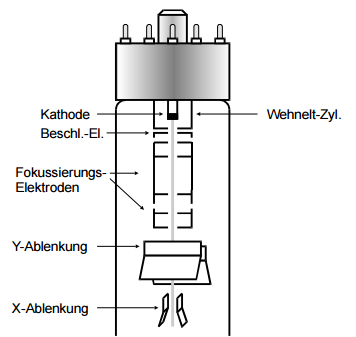
\includegraphics[width=0.5\textwidth]{krs.png}
 \caption{Queerschnitt einer Kathodenstrahlröhre.}
 \label{fig:krs}
\end{figure}
Die Röhre besteht im wesentlichen aus drei Komponenten, der "Elektronenkanone",
diese erzeugt, und beschleunigt freie Elektronen und
fokussiert den entstehenden Elektronenstrahl, einem Ablenksystem und einem Schirm.
Mittels Glühemission werden die freien Elektronen von einer Kathode, aus
einem Material mit kleiner Austrittsarbeit, erzeugt.
Die Kathode ist von einem sogenannten Wehnelt-Zylinder ummantelt, dieser enthält
eine Bohrung und weist ein negatives Potential auf, damit lässt sich die
Intensität des Elektronenstrahls steuern.
Eine Elektrode, mit hohem positivem Potential, befindet sich
vor dem Wehnelt-Zylinder. Die Elektrode beschleunigt diejenigen Elektronen,
welche den Wehnelt-Zylinder überwinden können, es folgt der Zusammenhang zur Beschleunigungsspannung $U_\mathrm{B}$:
\begin{align}
  \frac{m_\mathrm{0}v_\mathrm{z}^{2}}{2}=e_\mathrm{0}U_\mathrm{B} \label{eqn:beschleunigung}.
\end{align}
Das Strahlenbündel wird mit einer elektronischen Linse, mittels
inhomogener elekrischer Felder, auf einen Leuchtschirm fokussiert.
Die Brechkraft der Linse ist von der Spannung $U_\mathrm{c}$ abhängig.
Zwei Plattenpaare, deren Normalen senkrecht aufeinander stehen, bilden
das Ablenksystem. Beim Anlegen einer Spannung wirkt wegen des E-Feldes
eine Kraft auf den Elektronenstrahl und es kommt zur Ablenkung.
Diese Ablenkung ist sowohl von der Feldstärke als auch von der
Elektronengeschwindigkeit abhängig.

\subsubsection{Berechnung der Ablenkung im E-Feld}
Um den Zusammenhang zwischen Ablenkung $D$ und der Ablenkungsspannung
$U_\mathrm{D}$ herzuleiten, wird die Ablenkung zwischen zwei
Kondensatorplatten betrachtet, dargestellt in Abbildung \label{fig:platte}.
\begin{figure}
 \centering
 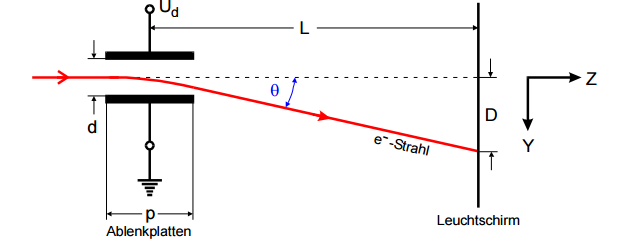
\includegraphics[width=0.6\textwidth]{kondensator.png}
 \caption{Ablenkung von Strahlen zwischen zwei geladenen Platten.}
 \label{fig:kondensator}
\end{figure}
Das elektrische Feld zwischen zwei Platten wird als homogen angesehen, wenn
$d<<p$ gilt.
Letzendlich ergibt sich mit Betrachtung der Komponenten der Geschwindigkeit
und des Winkels $\Theta$ die Ablenkung $D$ zu:
\begin{align}
 D=\frac{pLU_\mathrm{D}}{2dU_\mathrm{B}}.
\end{align}
Es herrscht eine Proportionalität zwischen $D$ und $U_\mathrm{D}$,
somit kann die Kathodenstrahlröhre zur Spannungsmessung genutzt werden.

<<<<<<< bc9e7461b69a9950378110056f0b3bca8428ba0a
\subsubsection{Der Kathodenstrahl-Oszillograph}
Eine Sägezahnspannung wird an das Ablenksystem in X-Richtung angelegt und die zu untersuchende Wechselspannung an das in Y-Richtung.
Stehen diese Spannungen in einem rationalen Verhältnis, so tAUCHT der Verlauf der Wechselspannung auf dem Schirm auf.

\subbsection{Elektronen im B-Feld}
Im Magnetfeld wird auf eine bewegte Ladung die Lorenzkraft,
||||||| merged common ancestors
\subbsection{Elektronen im B-Feld}
Im Magnetfeld wird auf eine bewegte Ladung die Lorenzkraft:
=======
\subsection{Elektronen im B-Feld}
Im Magnetfeld wird auf eine bewegte Ladung die Lorenzkraft:
>>>>>>> blaa
\begin{align}
\vec{F}\mathrm{L}=q\vec{v}\texttimes\vec{B},
\end{align}
ausgeübt. Damit $\vec{F}\mathrm{0} \neq 0 $ gilt, muss $\vec{v}$ senkrecht zum magnetischen Feld stehen.
Die Abbildung \ref{fig:kreis} zeigt, dass durch die Ablenkung das Elektron eine Kreisbahn beschreibt. Das Gleichgewicht zwischen Lorentzkraft und Zentrifugalkraft legt den
Radius der Kreisbahn fest:
\begin{align}
  r=\frac{m_\mathrm{0}v_\mathrm{0}}{e_\mathrm{0}B}\label{eqn:radius}.
\end{align}

\begin{figure}
 \centering
 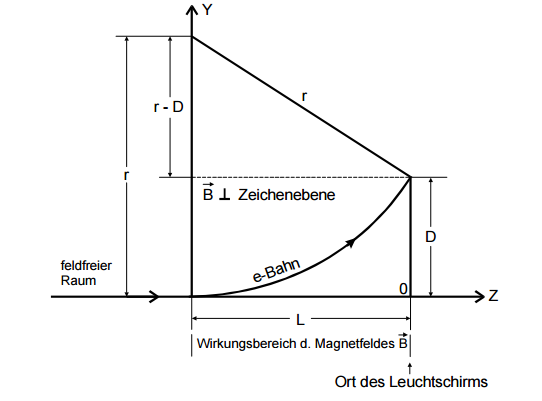
\includegraphics[width=0.6\textwidth]{b-feld.pdf}
 \caption{Darstellung der Strahlungsablenkung mittels Magnetfeld in einer Strahlröhre.}
 \label{fig:kreis}
\end{figure}

Um den Zusammenhang zwischen der Ablenkung $D$ und dem Magnetfeld $B$ zu bekommen, wird die Abbildung \ref{fig:kreis} erneut betrachtet.
Mit dem Satz von Pythagoras ergibt sich:
\begin{align}
  L^2+(r-D)^2=r^2
\end{align}
Mit der Gleichung \eqref{eqn:radius} und der Beziehung aus \eqref{eqn:beschleunigung}, folgt die Beziehung:
\begin{align}
  \frac{L^2+D^2}{2D}=\frac{1}{sqrt{8U_\mathrm{B}}}\sqrt{\frac{e_\mathr{0}}{m_\mathrm{0}}}B.
\end{align}
